\documentclass{article}
\usepackage{CJKutf8, graphicx}%导入CJKutf8包,并且激活中文、日文、韩文的uft8编码
\usepackage[utf8]{inputenc}

\title{短视频传输实验报告}
\author{计研173 \quad 陈雨兰 \quad 2017310787  \\ 计研173 \quad 蔡文静 \quad 2017210866}
\date{January 2018}

\begin{document}
\begin{CJK*}{UTF8}{gbsn}

\maketitle
\section{介绍}
该项目实现了从客户端到服务器端的短视频的快速上传。我们在UDP协议传输数据的基础上加上了数据解压缩、差错控制和数据包校验,实现了短视频的快速准确的传输。

\section{项目设计与分析}
\subsection{传输协议}
TCP和UDP是比较常用的传输协议。TCP提供可靠的通信传输,而UDP则常被用于让广播和细节控制交给应用的通信传输。
\subsubsection{TCP协议}
TCP是一种面向连接的协议,能提供可靠的传输服务,即TCP通过检验和、序列号、确认应答、重发控制、连接管理以及窗口控制等机制实现可靠性传输。TCP充分实现了数据传输时各种控制功能,可以进行丢包的重发控制,还可以对次序乱掉的分包进行顺序控制。但是这些功能也限制了TCP数据传输的速度,而且使得系统资源要求较高。
\subsubsection{UDP协议}

UDP是一个非连接的协议,传输数据之前源端和终端不建立连接,当它想传送时就简单地去抓取来自应用程序的数据,并尽可能快地把它扔到网络上。在发送端,UDP传送数据的速度仅仅是受应用程序生成数据的速度、计算机的能力和传输带宽的限制;在接收端,UDP把每个消息段放在队列中,应用程序每次从队列中读一个消息段。由于传输数据不建立连接,因此也就不需要维护连接状态,包括收发状态等,因此一台服务机可同时向多个客户机传输相同的消息。UDP信息包的标题很短,只有8个字节,相对于TCP的20个字节信息包的额外开销很小。UDP使用尽最大努力交付,即不保证可靠交付,因此主机不需要维持复杂的链接状态表(这里面有许多参数)。UDP是面向报文的。发送方的UDP对应用程序交下来的报文,在添加首部后就向下交付给IP层。既不拆分,也不合并,而是保留这些报文的边界,因此,应用程序需要选择合适的报文大小。

基于上述分析,TCP和UDP分别有如下几个特点:
\begin{itemize}
\item TCP面向连接;UDP面向无连接
\item TCP面向字节流;UDP面向报文
\item TCP首部开销大,有20字节,且占用资源较多;UDP首部开销小,只有8字节,且占用资源少
\item TCP提供可靠的服务,即,通过TCP连接传送的数据,无差错,不丢失,不重复,且按序到达;UDP尽最大努力交付,即不保证可靠交付;
\item UDP发送数据速度更快
\end{itemize}

\subsection{编码协议}

前向纠错策略(FEC)
每个数据包分为n个字
每个数据包的第i个字为一组,生成校验包
收到任意>=k个包,即可恢复k个数据包
冗余比例:r/k
改进:自适应的冗余比例;
丢失率过高时申请重发
\begin{figure}[h]
	\centering
	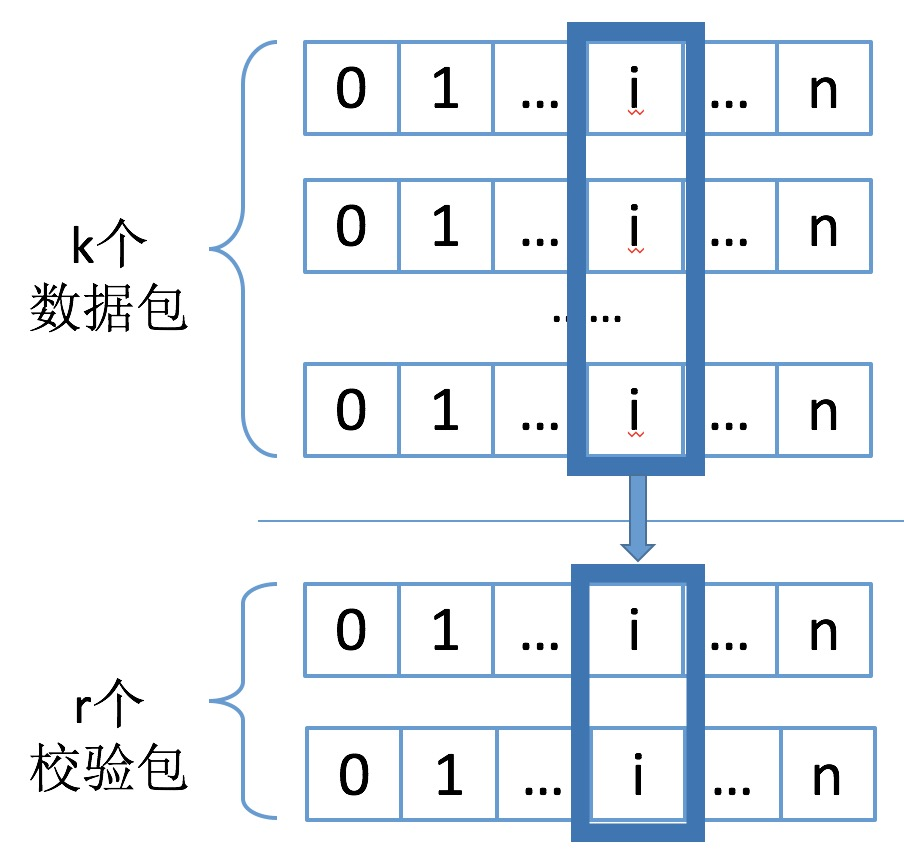
\includegraphics[width=2in]{FEC.jpg}
	\caption{前向纠错算法}
	\label{fig:FEC}
\end{figure}

\subsection{算法框架}
基于上述背景知识介绍,利用UDP的快速传输和开销小的特点,再加上差错控制等算法来保证可靠传输,我们设计了一个短视频的快速上传的项目。该项目框架图如图 \ref{fig:frame}所示。

\begin{figure}[h]
	\centering
	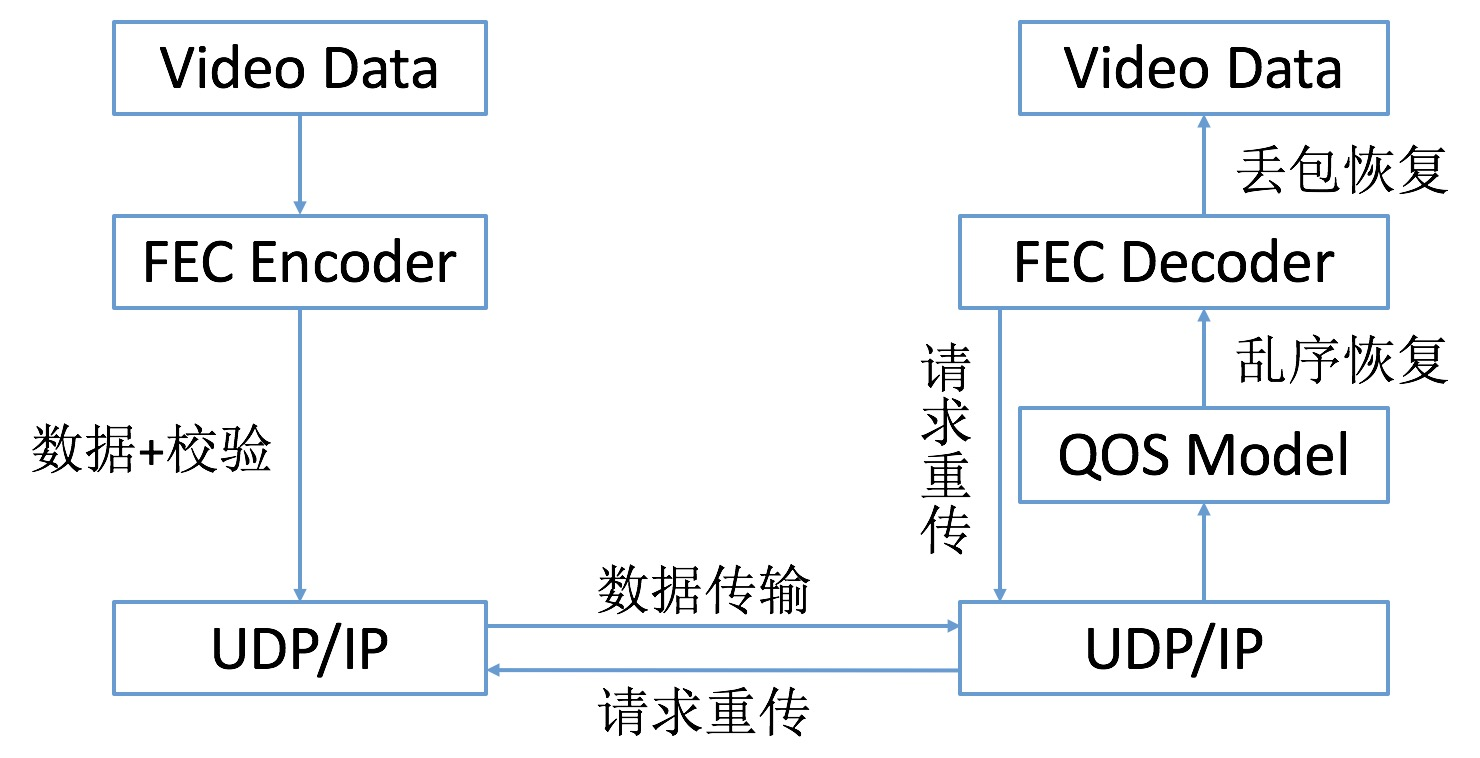
\includegraphics[width=3in]{frame.jpg}
	\caption{算法框架}
	\label{fig:frame}
\end{figure}

\subsection{项目实现}
我们使用eclipse进行android开发,使用java的socket编程实现udp协议的数据传输。
\subsubsection{实验环境}
\begin{itemize}
\item android. 客户端在android手机上实现了一个应用程序。该程序具有选择文件和传输文件的功能,界面图如图*所示,点击“选择文件”按钮选择想要上传的文件,选择文件后,点击“文件传输”,即开始进行文件上传。\textbf{android测试环境是小米5手机,android 7.0;该应用程序要求android版本最小是andorid 6.0}。
\item 服务器端。服务器端的实现是一个eclipse java程序。测试环境是windows 10 64位。在进行文件传输之前,需要先运行服务器端代码,服务器端即进行特定端口的监听,等待数据包的到来。 
\end{itemize}
\section{实验结果与分析}
\subsection{传输速度与冗余}
由于使用了前向纠错,算法的冗余度基本相当于前向纠错中校验包的比例。
\subsection{丢包修复能力}
在视频传输中,以固定比例随机丢包,测得算法的丢包比例和修复率之间的关系。
\end{CJK*}

\end{document}
